\documentclass[a4paper,12pt]{article}
\usepackage[utf8]{inputenc}

\usepackage[utf8]{inputenc}
\usepackage[T2A]{fontenc}
\usepackage[english,russian]{babel}
\usepackage{amsthm}
\usepackage{amsmath}
\usepackage{amssymb}
\usepackage{tikz}
\usepackage{textcomp}
\usepackage{marvosym}
\usepackage{ esint }
\usepackage{mathtext}
\usepackage{siunitx} % Required for alignment
\usepackage{subfigure}
\usepackage{multirow}
\usepackage{rotating}
\usepackage{afterpage}
\usepackage[arrowdel]{physics}
\usepackage{booktabs}
\setlength{\topmargin}{-0.5in}
\setlength{\textheight}{9.1in}
\setlength{\oddsidemargin}{-0.4in}
\setlength{\evensidemargin}{-0.4in}
\setlength{\textwidth}{7in}
\setlength{\parindent}{0ex}
\setlength{\parskip}{1ex}
\newcommand{\ndiv}{\hspace{-4pt}\not|\hspace{2pt}}
\usepackage{graphicx}
\usepackage{float}
\usepackage{wrapfig}
\usepackage{pgfplots}
\usepackage{caption}
\pgfplotsset{compat=1.16}
\graphicspath{ {./images/} }
\usepackage{graphicx}
\RequirePackage{caption}
\DeclareCaptionLabelSeparator{defffis}{ — }
\captionsetup{justification=centering,labelsep=defffis}
\usepackage{caption} \captionsetup[table]{labelsep=endash,justification=justified,singlelinecheck=false,font=normalsize}
\usepackage{amsfonts,mathtools}
\newcommand{\eds}{\ensuremath{ \mathscr{E}}}


\title{Лабораторная работа № 4.3.2\\Дифракция света на ультразвуковой волне в жидкости}
\author{Илья Прамский}
\date{Апрель 2024}

\begin{document}

\maketitle
\newpage
\section*{Введение}
\textbf{Цель:} изучение дифракции света на синусоидальной акустической решётке и наблюдение фазовой решётки методом тёмного
поля.

\textbf{Используются в работе:} оптическая скамья, осветитель, два длиннофокусных объектива, кювета с жидкостью, кварцевый излучатель
с микрометрическим винтом, генератор ультразвуковой частоты, линза, вертикальная нить на рейтере, микроскоп.

\section{Теоретическая справка}
При прохождении ультразвуковой волны через жидкость в ней возникают периодические неоднородности коэффициента преломления, создается фазовая решетка, которую мы считаем неподвижной ввиду малости скорости звука относительно скорости света. Показатель
	преломления n изменяется по закону:
	
	\begin{equation}\label{}
	n = n_0 (1 + m \cos \Omega x)
	\end{equation}
	
	Здесь $ \Omega = 2 \pi / \Lambda $ --- волновое число для ультразвуковой волны, $ m $ --- глубина модуляции $ n $ $ (m \ll 1 $).
	
	Положим фазу $ \phi $ колебаний световой волны на передней стенке кюветы равной нулю, тогда на задней поверхности она равна:
	
	\begin{equation}\label{}
	\phi  = k n L = \phi_0 (1 + m \cos \Omega x)
	\end{equation}
	
	Здесь $ L $ --- толщина жидкости в кювете, $ k = 2 \pi / \lambda $ --- волновое число для света.
	
	После прохождения через кювету световое поле есть совокупность плоских волн, распространяющихся под углами $ \theta $, соответствующими максимумам в дифракции Фраунгофера:
	
\begin{equation}\label{}	
	\Lambda \sin \theta_m = m \lambda
\end{equation}

Этот эффект проиллюстрирован на рисунке 1.

	Зная положение дифракционных максимумов, по формуле (1) легко определить длину ультразвуковой волны, учитывая малость $ \theta $: $ \sin \theta \approx \theta \approx l_m /F  $, где $ l_m $ --- расстояние от нулевого до последнего видимого максимума, $ F $ --- фокусное расстояние линзы. Тогда получим:
	
	\begin{equation}\label{}
	 \Lambda = m \lambda F/ l_m 
	\end{equation}
	Скорость ультразвуковых волн в жидкости, где $ \nu $ --- частота колебаний излучателя:
	
\begin{equation}\label{}
	v = \Lambda \nu 
\end{equation}

\begin{figure}[H]
	\center{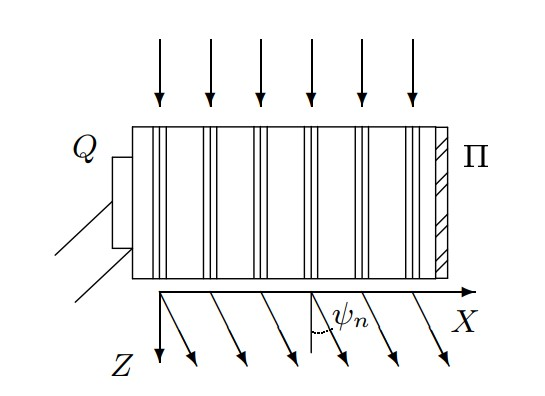
\includegraphics[scale=0.9]{1.jpg}}
  \caption{Эффект дифракции на ультразвуковой волне}
	\label{fig:image1}
\end{figure}

\section{Экспериментальная установка}
Источник света Л с помощью конденсора К проецируется на входную(коллиматорную) щель $S$. Входная щель ориентирована горизонтально и прикрыта красным светофильтром Ф. Коллиматорный объектив $\text{О}_1$ посылает параллельный пучок на кювету с водой $С$. Излучатель Q создаёт УЗ-волну. Параллельный пучок света, дифграгируя на стоячей звуковой волне, образует дифракционную картину в фокальной плоскости $F$ камерного объектива $\text{О}_{2}$. Картину можно наблюдать в микроскоп М.
\begin{figure}[H]
	\center{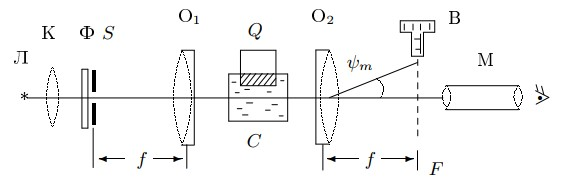
\includegraphics[scale=1]{2.jpg}}
  \caption{Схема экспериментальной установки}
	\label{fig:image1}
\end{figure}
\section{Ход работы}
\subsection*{Определение скорости ультразвука по дифракционной картине}
Для начала соберём и настроим схему, затем определим ноль для ширины щели(момент её открытия). Получился $d = 77 \pm 1$ мкм. Установим рабочую ширину в диапазоне $20-30$ мкм. Установили на $d = 100 \pm 1$ мкм, соответственно рабочая ширина щели равна $23 \pm 1$ мкм.

Чёткая дифракционную картина в поле зрения микроскопа получается при $\nu = 984,6 \pm 0,1$ кГц., оценим по порядку величину  длины УЗ-волны как удвоенное расстояние между наиболее чёткими дифракционными картинами. Две чёткие дифракционные картины получились на $19$ и $99$ соответственно(в ценах деления лимба излучателя, каждая из которых равна $10$ мкм). Получается $\Lambda = 2 \cdot (l_2 - l_1) = 1600 \pm 30$ мкм. Теперь оценим скорость звука в воде по формуле $(5)$. 
\[v = 1570 \pm 30 \text{м/с}\]
\\

Теперь определим координаты дифракционных полос для различных частот, затем по полученным данным построим графики зависимости $Y=Y(m)$, с помощью которых определим расстояние между соседними полосами, после чего при помощи формулы $(4)$, рассчитаем длину УЗ-волны, а также с помощью формулы $(5)$ найдём значение скорости звука в воде. $f = 28$ см, $\lambda = 6400 \pm 200 \text{\r{A}}$. $\sigma_Y = 4$ мкм.
\begin{table}[H]
	\centering
	\begin{tabular}{|c|c|c|c|}
	\hline
	\multicolumn{1}{|c|}{ } & $\nu_1 = 984,4$ кГц & $\nu_2 = 1002,0$ кГц & $\nu_3 = 1006,0$ кГц \\ \hline
	$m$ & $Y$, мкм  & $Y$, мкм & $Y$, мкм \\ \hline
	-3 & 4600 & 4652 & 4644 \\ \hline
	-2 & 4500 & 4516 & 4524 \\ \hline
	-1 & 4388 & 4392 & 4400 \\ \hline
  	 0 & 4248 & 4264 & 4264 \\ \hline
	 1 & 4120 & 4128 & 4124 \\ \hline
	 2 & 4004 & 4008 & 3988 \\ \hline
	 3 &	 3868 & 3884 & 3864 \\ \hline
	\end{tabular}
\end{table}

\begin{table}[H]
	\centering
	\begin{tabular}{|c|c|c|c|}
	\hline
	\multicolumn{1}{|c|}{ } & $\nu_4 = 1025,0$ кГц & $\nu_5 = 1600,0$ кГц & $\nu_6 = 4420,0$ кГц\\ \hline
	$m$ & $Y$, мкм &  $Y$, мкм &  $Y$, мкм \\ \hline
	-3 & \multicolumn{1}{|c|}{ } & \multicolumn{1}{|c|}{ } & \multicolumn{1}{|c|}{ } \\ \hline
	-2 & 4560 & \multicolumn{1}{|c|}{ } & \multicolumn{1}{|c|}{ } \\ \hline
	-1 & 4440 & 4460 & 4820 \\ \hline
  	 0 & 4268 & 4256 & 4260 \\ \hline
	 1 & 4092 & 4056 & 3700 \\ \hline
	 2 & 3948 & \multicolumn{1}{|c|}{ } & \multicolumn{1}{|c|}{ } \\ \hline
	 3 & \multicolumn{1}{|c|}{ } & \multicolumn{1}{|c|}{ } & \multicolumn{1}{|c|}{ } \\ \hline
	\end{tabular}
\end{table}



\begin{figure}[H]
	\centering
	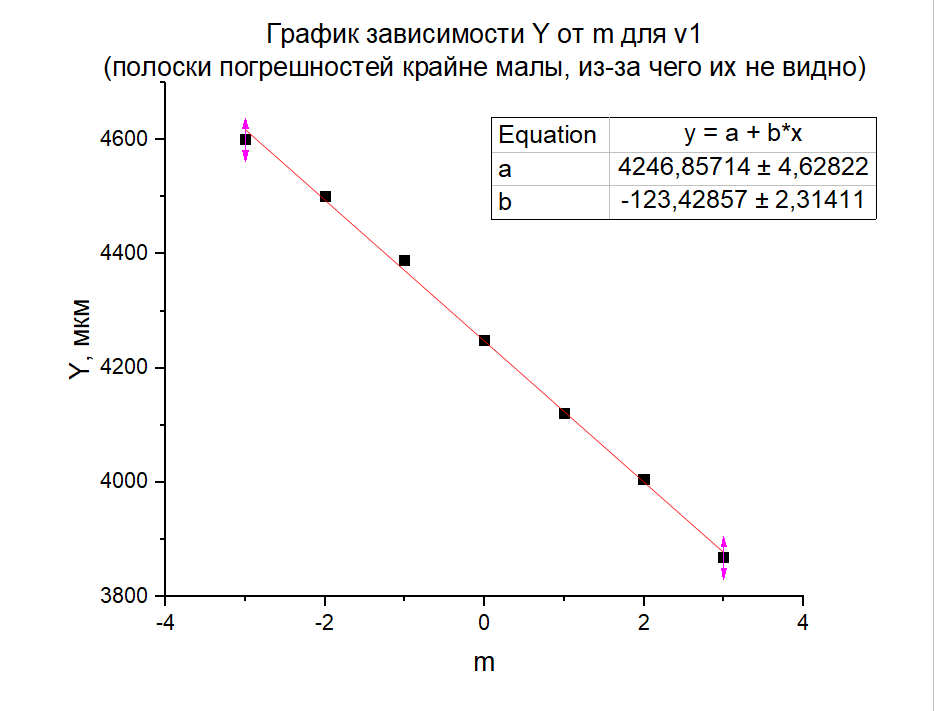
\includegraphics[width=0.8\linewidth]{graph1.png}
\end{figure}
\begin{figure}[H]
	\centering
	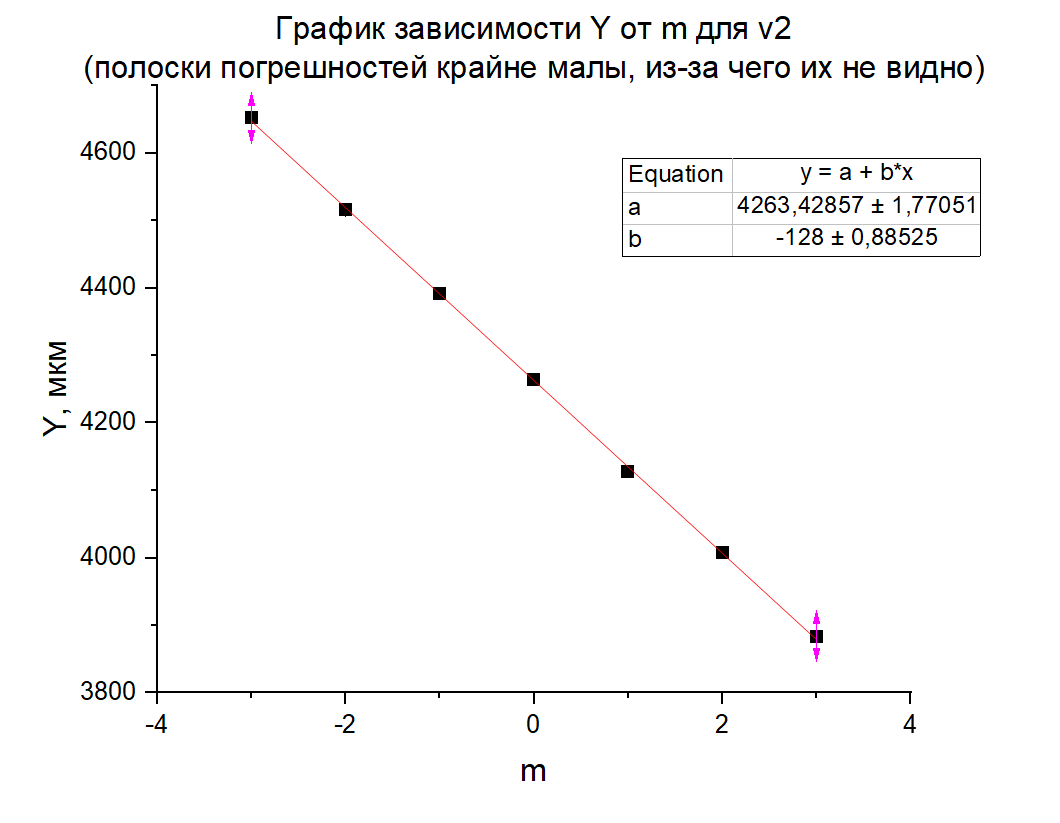
\includegraphics[width=0.8\linewidth]{graph2.png}
\end{figure}
\begin{figure}[H]
	\centering
	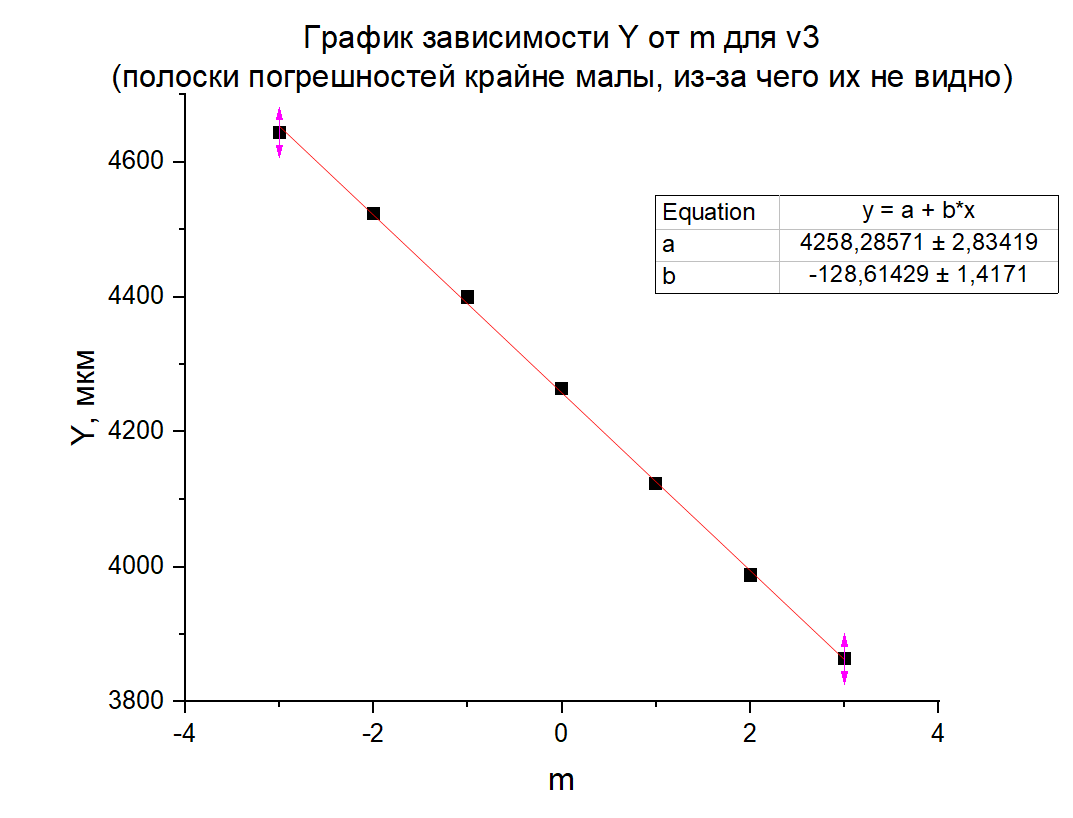
\includegraphics[width=0.8\linewidth]{graph3.png}
\end{figure}
\begin{figure}[H]
	\centering
	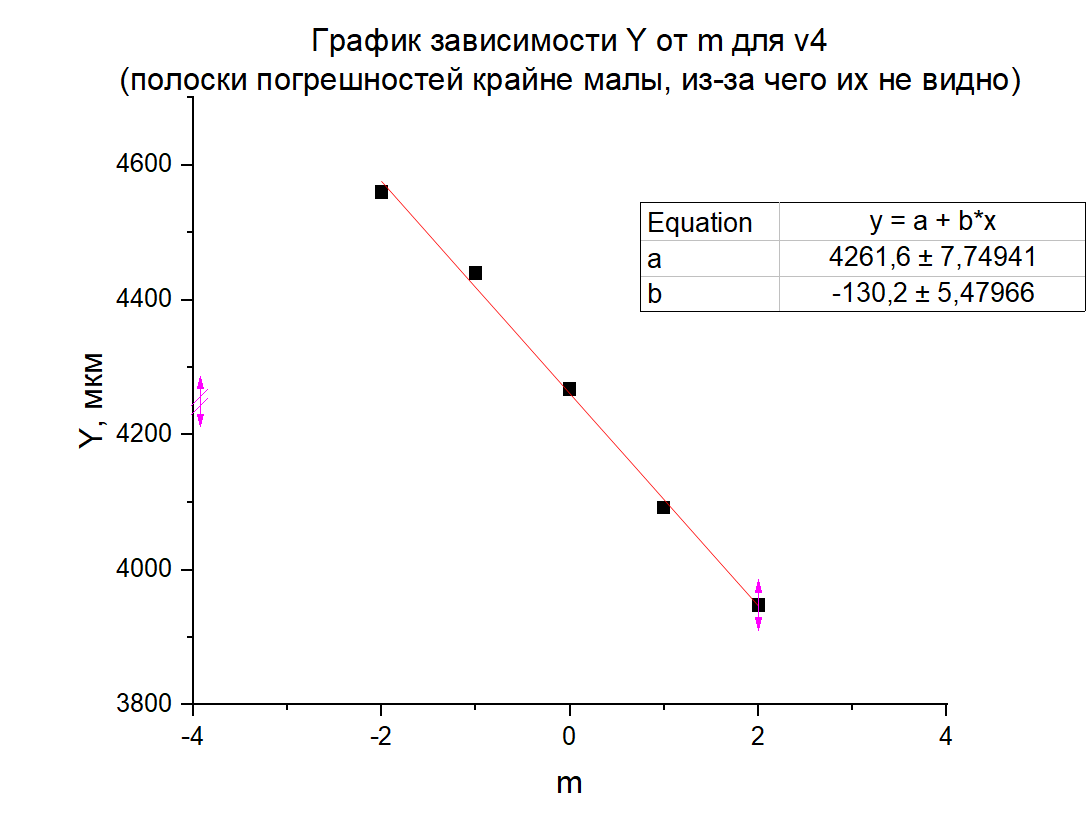
\includegraphics[width=0.8\linewidth]{graph4.png}
\end{figure}
\begin{figure}[H]
	\centering
	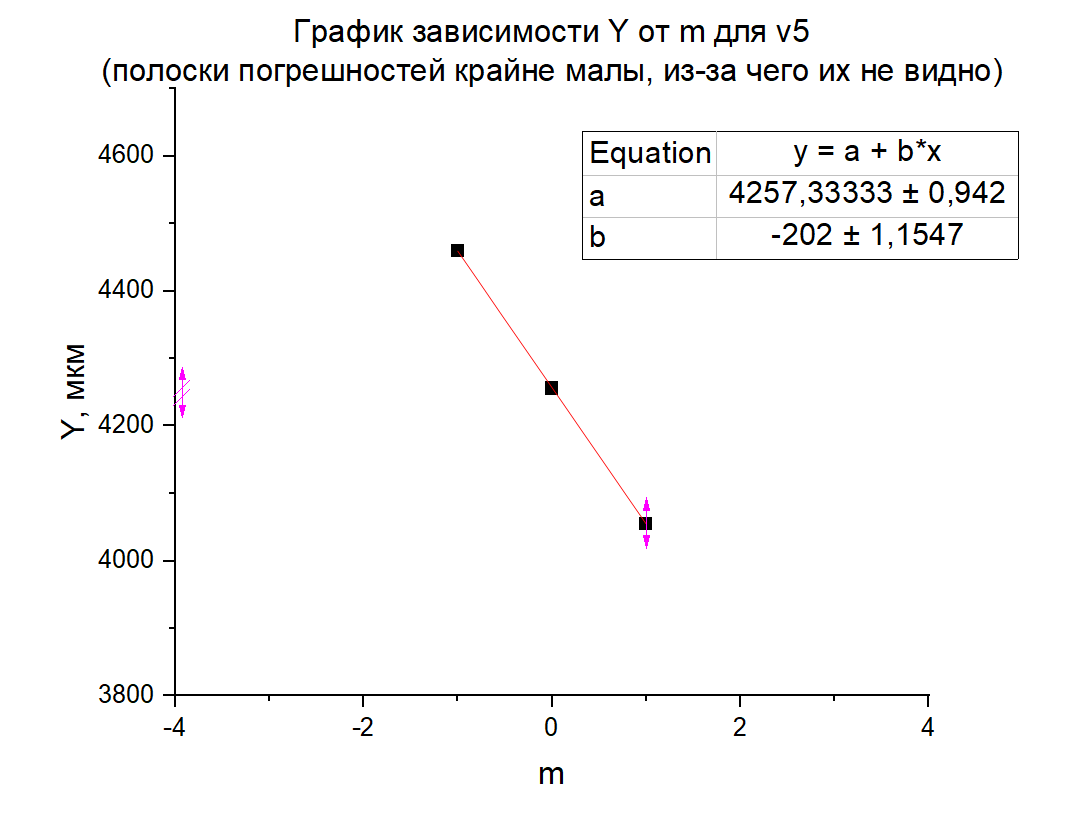
\includegraphics[width=0.8\linewidth]{graph5.png}
\end{figure}
\begin{figure}[H]
	\centering
	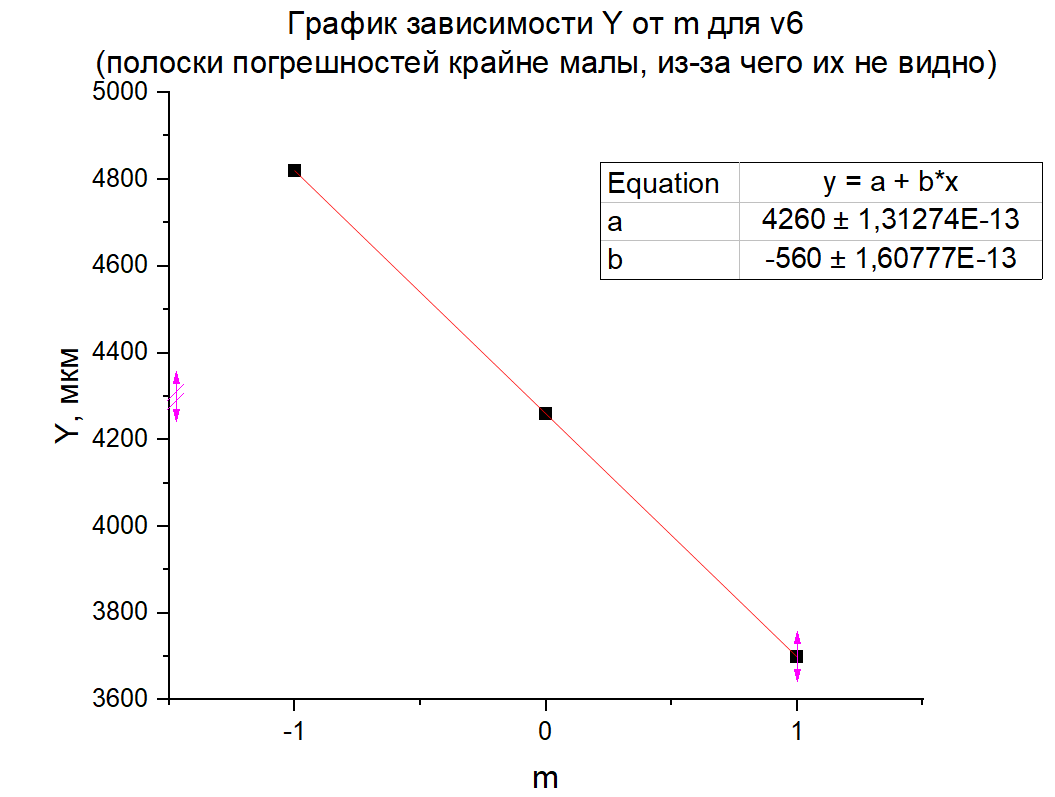
\includegraphics[width=0.8\linewidth]{graph6.png}
\end{figure}

Полученные значения занесём в таблицу
\begin{table}[H]
	\begin{tabular}{|c|c|c|c|c|c|c|c|}
	\hline
	$\nu$, кГц & $\Delta l$, мкм & $\sigma_{\Delta l}$, мкм & $\Lambda$, мкм & $\sigma_{\Lambda}$, мкм & $V$, м/с & $\sigma_V$, м/c \\ \hline
	984,4 & 123 & 2 & 1457 & 50 & 1434 & 51\\ \hline
	1002,0 & 128,0 & 0,9 & 1400 & 40 & 1403 & 45\\ \hline
	1006,0 & 128,6 & 1,4 & 1393 & 50 & 1402 & 46 \\ \hline
	1025,0 & 130 & 5 & 1378 & 70 & 1413 & 70 \\ \hline
	1060,0 & 202,0 & 1,2 & 887 & 30 & 1419 & 45 \\ \hline
	4420,0 & 560 & 0 & 320 & 10 & 1414 & 44 \\ \hline
	
	\end{tabular}
\end{table}

Получается средняя скорость звука в воде исходя из проведённых измерений равна $V = 1414 \pm 21$ м/с. Теоретическое же значение равно 1403 м/с, что находится достаточно близко к полученному на опыте(даже лежит в пределах погрешности экспериментального значения).
\subsection*{Определение скорости ультразвука методом тёмного поля}
Теперь поставим между щелью и микроскопом дополнительную линзу, затем также установим в воде пластинку с калибровочной сеткой, сторона квадрата у которой равна 1 мм. При помощи этой сетки откалибруем окулярную шкалу микроскопа. Так, на 1 квадрат, приходится 23 штриха окулярной шкалы микроскопа, значит цена деления равна $\frac{1}{23}$ мм. 

Также закроем нулевой дифракционный максимум проволочкой. Теперь, меняя частоту, найдём наиболее чёткие картины звуковой решётки, затем измерим координаты первой и последней тёмных полос и количество светлых промежутков между ними. Результаты измерений занесём в таблицу, с их помощью найдём длину УЗ-волны $\Lambda$, учитывая удвоение числа наблюдаемых полос. Построим график зависимости $\Lambda = f(\frac{1}{\nu}$, при помощи которого(по наклону) определим скорость звука в воде.($x_1, x_n$ координаты первой и последней полосы соответственно). Также в таблице единица "дел" отвечает за 25 штрихов окулярной шкалы.

\begin{table}[H]
	\centering
	\begin{tabular}{|c|c|c|c|c|c|c|}
	\hline
	$\nu$, кГц & $x_1$, дел & $x_n$, дел & $\Delta x$, мм & $m$ & $\Lambda$, мм & $\sigma_{\Lambda}$, мм  \\ \hline
	940 & -1 & 7,73 & 9,49 & 13 & 1,46 & 0,01 \\ \hline
	975 & -1 & 7,37 & 9,10 & 13 & 1,40 & 0,01 \\ \hline
	1010 & -1 & 7,83 & 9,60 & 14 & 1,37 & 0,01 \\ \hline
	1043 & -1 & 7,98 & 9,76 & 15 & 1,30& 0,008 \\ \hline	
	\end{tabular}
\end{table}

\begin{figure}[H]
	\centering
	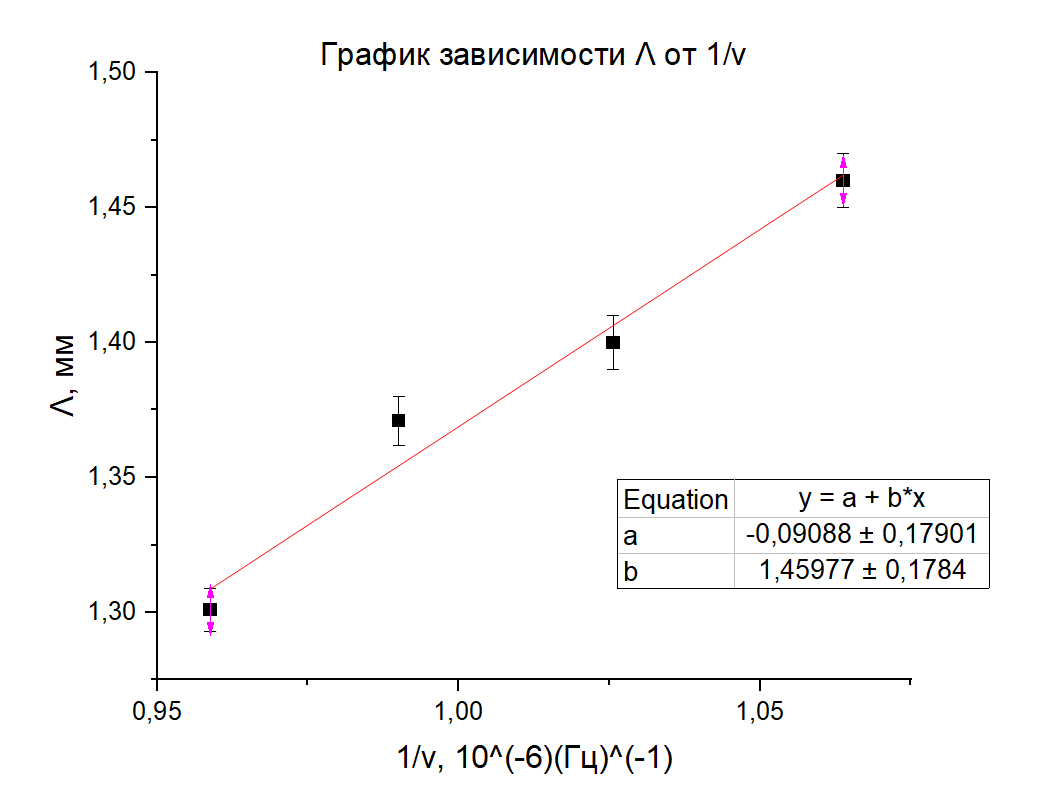
\includegraphics[scale=0.8]{graph7.png}
\end{figure}

Получается из графика $V = 1459 \pm 178$ м/c, что также охватывает в свой диапазон теоретическое значение.

\section{Вывод}
В ходе данной работы была изучена дифракция на акустической решётке, с её помощью различными способами была как и оценена скорость звука в воде($v = 1570 \pm 30$ м/с), так и вычислена более точно при помощи формул (4) и (5) и исследования зависимости координат дифракционных полос от порядка максимума при различных частотах, в результате чего было получено значение $v = 1414 \pm 21$ м/c. Также во время выполнения удалось получить чёткие картины звуковой решётки, с помощью которых также была вычислена скорость звука в воде(получившееся значение равно $v = 1459 \pm 178$ м/c). Теоретическое же значение равно 1403 м/c, что согласуется с полученными нами данными. Самым дальним от табличного получилось первое значение, что можно объяснить недостаточной точностью этого способа вычисления(в задании просили оценить этим способом значение скорости звука в воде).  
\end{document}